\begin{center}
  \subsection*{Sample Sizes (Denoted as N):}
  \(N_{\ONE\C}\)~=~\BOX{\boxed{11}}{R},~~\(N_{\TWO\C}\)~=~\BOX{\boxed{9}}{G},~~\(N_{\THR\C}\)~=~\BOX{\boxed{8}}{B},~~\(N_{\FOR\C}\)~=~\BOX{\boxed{11}}{A}
  \subsection*{Average of Change (Denoted as MEAN):}
  \(\overline{X}_{\ONE\C} =\frac{X_1 +\cdots + X_{11}}{N_{\ONE\C}}\),\\
  =~\BOX{\boxed{9.82}}{R}\\\text{}\\
  \(\overline{X}_{\TWO\C} =\frac{X_{12} +\cdots + X_{23}}{N_{\TWO\C}}\),\\
  =~\BOX{\boxed{11.10}}{G}\\\text{}\\
  \(\overline{X}_{\THR\C} =\frac{X_{24} +\cdots + X_{32}}{N_{\THR\C}}\),\\
  =~\BOX{\boxed{13.33}}{B}\\\text{}\\
  \(\overline{X}_{\FOR\C} =\frac{X_{33} +\cdots + X_{41}}{N_{\FOR\C}}\),\\
  =~\BOX{\boxed{10.55}}{A}\\
  \subsection*{Standard Deviations (Denoted as SD):}
  \(\sigma_{\ONE\C} =\sqrt{\frac{\left|X_1 - \overline{X}_{\FOR\C}\right|^2 +\cdots +\left|X_{11} - \overline{X}_{\FOR\C}\right|^2}{N_{\ONE\C} - 1}}\),\\
  =~\BOX{\boxed{3.03}}{R}\\\text{}\\
  \subsection*{Standard Errors (Denoted as \(\pm \)SE):}
  \(\epsilon_{\ONE\C} =\frac{\sigma_{\ONE\C}}{\sqrt{N_{\ONE\C}}}\),\\
  =~\BOX{\boxed{0.9127}}{R}
\end{center}
\newpage
\begin{center}
  % BLUE, GREEN, RED, PURPLE
  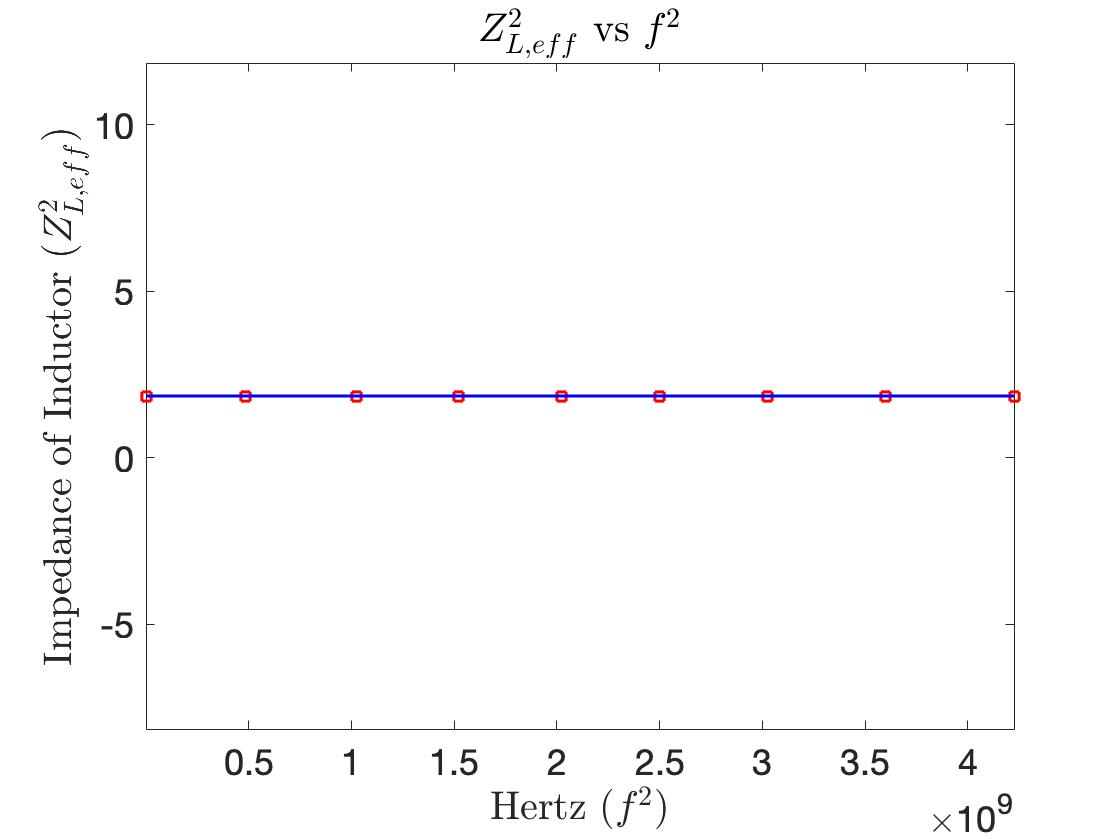
\includegraphics[width=\textwidth]{graph.jpg}
  \fbox{\begin{minipage}{50em}\text{}
    \begin{enumerate}
      \item What was the mean \(\pm \) standard error of coral growth (= change mg/cm2) at each of the four temperature categories?
      \begin{itemize}
        \item~~\quad{\(\ONE\C \)}~=~\BOX{\boxed{09.82~(mg/cm^2)~\pm~0.91}}{R}
        \item~~\quad{\(\TWO\C \)}~=~\BOX{\boxed{11.10~(mg/cm^2)~\pm~0.89}}{G}
        \item~~\quad{\(\THR\C \)}~=~\BOX{\boxed{13.33~(mg/cm^2)~\pm~1.04}}{B}
        \item \(\FOR\C \)~=~\BOX{\boxed{10.55~(mg/cm^2)~\pm~0.98}}{A}
      \end{itemize}
      \item What would happen if global climate change causes the average seawater temperature to increase to 30?
      \begin{itemize}
        \item
      \end{itemize}
      \text{}
    \end{enumerate}
  \end{minipage}}
\end{center}